\chapter{The force betwen nucleons}
Even before describing any further experiments to study the force between two nucleons, we can already guess at a few of the properties of the nucleon-nucleon force:\\
\begin{enumerate}
	\item At short distances it is stronger than the Coulomb force: the nuclear force can overcome the Coulomb repulsion of protons in the nucleus.
	\item At long distances, of the order of atomic sizes, the nuclear force is negligibly feeble: the interactions among nuclei in a molecule can be understood based only on the Coulomb force.
	\item Some particles are immune from the nuclear force: there is no evidence from atomic structure, for example. that electrons feel the nuclear force at all.
	\item The nucleon-nucleon force seems to be nearly independent of whether the nucleons are neutrons or protons. This property is called charge independence.
	\item The nucleon-nucleon force depends on whether the spins of the nucleons are parallel or antiparallel.
	\item The nucleon-nucleon force includes a repulsive term. which keeps the nucleons at a certain average separation.
	\item The nucleon-nucleon force has a noncentral or tensor component. This part of the force does not conserve orbital angular momentum. which is a constant of the motion under central forces.
\end{enumerate}
\section{Properties of nuclear force(in detail)}
\subsection{ The Nucleon - Nucleon Interaction is Strongly Spin Dependent}
Until now we neglected the fact that both neutron and proton possess a spin. The question remains how the spin influences the interaction between the two particles. The total angular momentum for the deuteron (or in general for a nucleus) is usually denoted by $I$. Here it is given by
$$
\hat{\vec{I}}=\hat{\vec{L}}+\hat{\vec{S}}_{p}+\hat{\vec{S}}_{n}
$$
For the bound deuteron state $l=0$ and $\hat{\vec{I}}=\hat{\vec{S}}_{p}+\hat{\vec{S}}_{n}=\hat{\vec{S}}$. A priori we can have $\hat{\vec{S}}=0$ or 1 (recall the rules for addition of angular momentum, here $\hat{\vec{S}}_{p, n}=\frac{1}{2}$ ).
There are experimental signatures that the nuclear force depends on the spin. In fact the deuteron is only found with $\hat{\vec{S}}=1$ (meaning that this configuration has a lower energy).\\
\par The simplest form that a spin-dependent potential could assume is $V_{\text {spin }} \propto \hat{\vec{S}}_{p} \cdot \hat{\vec{S}}_{n}$ (since we want the potential to be a scalar). The coefficient of proportionality $V_{1}(r) / \hbar^{2}$ can have a spatial dependence. Then, we guess the form for the spin-dependent potential to be $V_{\text {spin }}=V_{1}(r) / \hbar^{2} \hat{\vec{S}}_{p} \cdot \hat{\vec{S}}_{n}$. What is the potential for the two possible configurations of the neutron and proton spins?
The configuration are either $\hat{\vec{S}}=1$ or $\hat{\vec{S}}=0$. Let us write $\hat{\vec{S}}^{2}=\hbar S(S+1)$ in terms of the two spins:
$$
\hat{\vec{S}}^{2}=\hat{\vec{S}}_{p}^{2}+\hat{\vec{S}}_{n}^{2}+2 \hat{\vec{S}}_{p} \cdot \hat{\vec{S}}_{n}
$$
The last term is the one we are looking for:
$$
\hat{\vec{S}}_{p} \cdot \hat{\vec{S}}_{n}=\frac{1}{2}\left(\hat{\vec{S}}^{2}-\hat{\vec{S}}_{p}^{2}-\hat{\vec{S}}_{n}^{2}\right)
$$
Because $\hat{S}^{2}$ and $\hat{\vec{S}}_{p}^{2}, \hat{\vec{S}}_{n}^{2}$ commute, we can write an equation for the expectation values wrt eigenfunctions of these operators 10 :
$$
\left\langle\hat{\vec{S}}_{p} \cdot \hat{\vec{S}}_{n}\right\rangle=\left\langle S, S_{p}, S_{n}, S_{z}\left|\hat{\vec{S}}_{p} \cdot \hat{\vec{S}}_{n}\right| S, S_{p}, S_{n}, S_{z}\right\rangle=\frac{\hbar^{2}}{2}\left(S(S+1)-S_{p}\left(S_{p}+1\right)-S_{n}\left(S_{n}+1\right)\right)
$$
since $S_{p, n}=\frac{1}{2}$, we obtain
$$
\left\langle\hat{\vec{S}}_{p} \cdot \hat{\vec{S}}_{n}\right\rangle=\frac{\hbar^{2}}{2}\left(S(S+1)-\frac{3}{2}\right)=\begin{array}{ll}
+\frac{\hbar^{2}}{4} & \text { Triplet State, }\left|S=1, \frac{1}{2} \frac{1}{2}, m_{z}\right\rangle \\
-\frac{3 \hbar^{2}}{4} & \text { Singlet State, }\left|S=0, \frac{1}{2}, \frac{1}{2}, 0\right\rangle
\end{array}
$$
If $V_{1}(r)$ is an attractive potential $(<0)$, the total potential is $\left.V_{n u c}\right|_{S=1}=V_{T}=V_{0}+\frac{1}{4} V_{1}$ for a triplet state, while its strength is reduced to $\left.V_{n u c}\right|_{S=0}=V_{S}=V_{0}-\frac{3}{4} V_{1}$ for a singlet state. How large is $V_{1}$ ?
We can compute $V_{0}$ and $V_{1}$ from knowing the binding energy of the triplet state and the energy of the unbound virtual state of the singlet (since this is very close to zero, it can still be obtained experimentally). We have $E_{T}=-2.2 \mathrm{MeV}$ (as before, since this is the experimental data) and $E_{S}=77 \mathrm{keV}$. Solving the eigenvalue problem for a square well, knowing the binding energy $E_{T}$ and setting $E_{S} \approx 0$, we obtain $V_{T}=-35 \mathrm{MeV}$ and $V_{S}=-25 \mathrm{MeV}(\mathrm{Notice}$ that of course $V_{T}$ is equal to the value we had previously set for the deuteron potential in order to find the correct binding energy of $2.2 \mathrm{MeV}$, we just -wrongly- neglected the spin earlier on). From these values by solving a system of two equations in two variables:
$$
\left\{\begin{array}{l}
V_{0}+\frac{1}{4} V_{1}=V_{T} \\
V_{0}-\frac{3}{4} V_{1}=V_{S}
\end{array}\right.
$$
we obtain $V_{0}=-32.5 \mathrm{MeV} V_{1}=-10 \mathrm{MeV}$. Thus the spin-dependent part of the potential is weaker, but not negligible.
\subsection{The Internucleon Potential Includes a Noncentral Term, Known as a Tensor Potential}
Evidence for the tensor force comes primarily from the observed quadrupole moment of the ground state of the deuteron. An s-state $(\ell=0)$ wave function is spherically symmetric; the electric quadrupole moment vanishes. Wave functions with mixed $\ell$ states must result from noncentral potentials. For a single nucleon, the choice of a certain direction in space is obviously arbitrary; nucleons do not distinguish north from south or east from west. The only reference direction for a nucleon is its spin, and thus only terms of the form $s \cdot r$ or $s \times \boldsymbol{r}$, which relate $r$ to the direction of $s$, can contribute. To satisfy the requirements of parity invariance, there must be an even number of factors of $r$, and so for two nucleons the potential must depend on terms such as $\left(s_{1} \cdot \boldsymbol{r}\right)\left(s_{2} \cdot \boldsymbol{r}\right)$ or $\left(s_{1} \times \boldsymbol{r}\right) \cdot\left(s_{2} \times \boldsymbol{r}\right)$.
Using vector identities we can show that the second form can be written in terms of the first and the additional term $s_{1} \cdot s_{2}$, which we already included in $V(r)$. Thus without loss of generality we can choose the tensor contribution to the internucleon potential to be of the form $V_{\mathrm{T}}(r) S_{12}$, where $V_{\mathrm{T}}(r)$ gives the force the proper radial dependence and magnitude, and
$$S_{12}=3\left(s_{1} \cdot r\right)\left(s_{2} \cdot r\right) / r^{2}-s_{1} \cdot s_{2}$$
which gives the force its proper tensor character and also averages to zero over all angles.
\subsection{ The Nucleon - Nucleon Force Is Charge Symmetric}
This means that the proton-proton interaction is identical to the neutron-neutron interaction, after we correct for the Coulomb force in the proton-proton system. Here "charge" refers to the character of the nucleon (proton or neutron) and not to electric charge. Evidence in support of this assertion comes from the equality of the pp and nn scattering lengths and effective ranges. Of course. the pp parameters must first be corrected for the Coulomb interaction. When this is done, the resulting singlet pp parameters are
 \begin{align*}
	&a=-17.1 \pm 0.2 \mathrm{fm} \\
	&r_{0}=2.84 \pm 0.03 \mathrm{fm}
\end{align*}
These are in very good agreement with the measured nn parameters ( $a=-16.6$ $\pm 0.5 \mathrm{fm}, r_{0}=2.66 \pm 0.15 \mathrm{fm}$ ). which strongly supports the notion of charge symmetry.
\subsection{The Nucleon - Nucleon Force Is Nearly Charge Independent}
After correcting for the electromagnetic interaction, the forces between nucleons (pp, nn, or np) in the same state are almost the same.
The force between a pair of protons, a pair of neutrons, and a pair of neutrons and protons are equal.
$$
F(n-n)=F(p-p)=F(n-p)
$$
The net force between pair of neutrons and a pair of neutron and proton is equal. This is slightly greater than the force between pair of protons because force between protons is reduced due to electrostatic repulsion
Net force $F(n-n)=$ Net force $F(n-p)>$ Net force $F(p-p)$
\subsection{The Nucleon-Nucleon Interaction Becomes Repulsive at Short Distances}
This conclusion follows from qualitative considerations of the nuclear density: as we add more nucleons, the nucleus grows in such a way that its central density remains roughly constant, and thus something is keeping the nucleons from crowding too closely together.
\section{The Deuteron}
A deuteron ( ${ }^{2} \mathrm{H}$ nucleus) consists of a neutron and a proton. (A neutral atom of ${ }^{2} \mathrm{H}$ is called deuterium.) It is the simplest bound state of nucleons and therefore gives us an ideal system for studying the nucleon-nucleon interaction. For nuclear physicists, the deuteron should be what the hydrogen atom is for atomic physicists. Just as the measured Balmer series of electromagnetic transitions between the excited states of hydrogen led to an understanding of the structure of hydrogen, so should the electromagnetic transitions between the excited states of the deuteron lead to an understanding of its structure. Unfortunately. there are no excited states of the deuteron-it is such a weakly bound system that the only "excited states" are unbound systems consisting of a free proton and neutron.
\subsection{Binding Energy}
The binding energy of the deuteron is a very precisely measured quantity. which can be determined in three different ways.\\
\textbf{First method}\\
The following determinations have been made (we use the symbol $\mathrm{D}$ for ${ }^{2} \mathrm{H}$ ):
$$
m\left(\mathrm{C}_{6} \mathrm{H}_{12}\right)-m\left(\mathrm{C}_{6} \mathrm{D}_{6}\right)=(9.289710 \pm 0.000024) \times 10^{-3} \mathrm{u}
$$
and
$$
m\left(C_{5} D_{12}\right)-m\left(C_{6} D_{6}\right)=(84.610626 \pm 0.000090) \times 10^{-3} \mathrm{u}
$$
From the first difierence we find. using $1.007825037 \mathrm{u}$ for the ${ }^{1} \mathrm{H}$ mass.
$$
m\left({ }^{2} \mathrm{H}\right)=2.014101789 \pm 0.000000021 \mathrm{u}
$$
and from the second.
$$
m\left({ }^{2} \mathrm{H}\right)=2.014101771 \pm 0.000000015 \mathrm{u}
$$
These precise values are in very good agreement.\\
\textbf{second method}\\
 And using the measured ${ }^{1} \mathrm{H}$ and neutron masses we can find the binding energy
 $$
 B=\left[m\left({ }^{1} \mathrm{H}\right)+m(\mathrm{n})-m\left({ }^{2} \mathrm{H}\right)\right] c^{2}=2.22463 \pm 0.00004 \mathrm{MeV}
 $$
 \textbf{Third method}\\
 We can also determine this binding energy directly by bringing a proton and a neutron together to form ${ }^{2} \mathrm{H}$ and measuring the energy of the $\gamma$-ray photon that is emitted:
 $$
 { }^{1} \mathrm{H}+\mathrm{n} \rightarrow{ }^{2} \mathrm{H}-\gamma
 $$
 The deduced binding energy. which is equal to the observed energy of the photon less a small recoil correction. is $2.224589 \pm 0.000002 \mathrm{MeV}$, in excellent agreement with the mass spectroscopic value. 
 \subsection{Spin and parity}
 The total angular momentum $I$ of the deuteron should have three components: the individual spins $s_{\mathrm{n}}$ and $s_{\mathrm{p}}$ of the neutron and proton (each equal to $\frac{1}{2}$ ), and the orbital angular momentum $\ell$ of the nucleons as they move about their common center of mass:
 $$
 \boldsymbol{I}=\boldsymbol{s}_{\mathrm{n}}+s_{\mathrm{p}}+\ell
 $$
 When we solved the Schrödinger equation for the deuteron, we assumed $\ell=0$ in analogy with the lowest bound state (the $1 \mathrm{~s}$ state) in atomic hydrogen. The measured spin of the deuteron is $I=1$. Since the neutron and proton spins can be either parallel (for a total of 1 ) or antiparallel (for a total of zero), there are four ways to couple $s_{\mathrm{n}} . s_{\mathrm{p}}$. and $t$ to get a total $I$ of 1 :\\\\
 (a) $s_{n}$ and $s_{p}$ parallel with $\ell=0$.\\
 (b) $s_{n}$ and $s_{p}$ antiparallel with $l=1$.\\
 (c) $s_{\mathrm{n}}$ and $s_{\mathrm{p}}$ parallel with $l=1$.\\
 (d) $s_{n}$ and $s_{p}$ parallel with $l=2$.\\
 Another property of the deuteron that we can determine is its parity (even or odd). the behavior of its wave function when $r \rightarrow-r$. By studving the reactions involving deuterons and the property of the photon emitted during the formation of deuterons. we know that its parity is even. The observed even parity allows us to eliminate the combinations of spins that include $t=1$. leaving $\ell=0$ and $t=2$ as possibilities. The spin and parity of the deuteron are therefore consistent with $t=0$ as we assumed. but of course we cannot vet exclude the possibility of $t=2$.
 \subsection{Magnetic dipole moment}
 We knoe that the spin and orbital contributions to the magnetic dipole moment. If the $t=0$ assumption is correct. there should be no orbital contribution to the magnetic moment. and we can assume the total magnetic moment to be simply the combination of the neutron and proton magnetic moments:
 \begin{align*}
 \mu &=\mu_{n}+\mu_{p} \\
 &=\frac{g_{s n} \mu_{N}}{\hbar} s_{n}+\frac{g_{s p} \mu}{\hbar} s_{p}
 \end{align*}
 where $g_{\text {on }}=-3.826084$ and $g_{s p}=5.585691$. we take the observed magnetic moment to be the z component of $\mu$ when the spins have their maximum value $\left(+\frac{1}{2} \hbar\right)$ :
 \begin{align*}
 \mu &=\frac{1}{2} \mu_{N}\left(g_{s n}+g_{s p}\right) \\
 &=0.879804 \mu_{N}
 \end{align*}
 The observed value is $0.8574376 \pm 0.0000004 \mu_{\mathrm{N}}$, in good but not quite exact agreement with the calculated value. The small discrepancy can be ascribed to any of a number of factors, such as contributions from the mesons exchanged between the neutron and proton; in the context of the present discussion, we can assume the discrepancy to arise from a small mixture of $\mathrm{d}$ state $(\ell=2)$ in the deuteron wave function:
 $$\psi=a_{\mathrm{s}} \psi(\ell=0)+a_{\mathrm{d}} \psi(\ell=2)$$
Calculating the magnetic moment from this wave function gives
$$
\mu=a_{\mathrm{s}}^{2} \mu(\ell=0)+a_{\mathrm{d}}^{2} \mu(\ell=2)
$$
where $\mu(\ell=0)$ is the value calculated above and $\mu(\ell=2)=\frac{1}{4}\left(3-g_{s \mathrm{p}}\right.$ $\left.-g_{s \mathrm{n}}\right) \mu_{\mathrm{N}}$ is the value calculated for a d state. The observed value is consistent with $a_{\mathrm{s}}^{2}=0.96, a_{\mathrm{d}}^{2}=0.04$; that is, the deuteron is $96 \% \ell=0$ and only $4 \% \quad \ell=2$. The assumption of the pure $t=0$ state, which we made in calculating the well depth, is thus pretty good but not quite exact.
\subsection{Electric Quadrupole Moment}
The bare neutron and proton have no electric quadrupole moment. and so any measured nonzero value for the quadrupole moment must be due to the orbital motion. Thus the pure $t=0$ wave function would have a vanishing quadrupole moment. The observed quadrupole moment is
$$
Q=0.00288 \pm 0.00002 \mathrm{~b}
$$
which. while small by comparison with many other nuclei. is certainly not zero.
\section{Nucleon Nucleon potential}
The exact mathematical form of the interaction potential is not known.One approximate such a strong short range spherically symmetric potential by one of the following expressions.
\begin{enumerate}
	\item \textbf{Rectangular well potential}\\
	\begin{align*}
		V &=-V_{0} \text { for } r \leq b \\
		&=0 \text { for } r>b
	\end{align*}
	Often used in calculation, where $V_{0}>0$ and $b$ is the radius of the well.
	\item \textbf{Expotential Well Potential}
	$$
	V=-V_{0} \exp \left(-\frac{r}{b}\right)
	$$
	\item \textbf{Yukuwa Potetial}
	$$
	V=-\left\{\frac{V_{0}}{r / b}\right\} \exp \left(-\frac{r}{b}\right)
	$$
	\item \textbf{Wooden -Saxon Potential}
	$$
	V=-\frac{V_{0}}{\left[1+\exp \left\{-\frac{(r-b)}{c}\right\}\right]}
	$$
	Where $c$ is constant and representing the skin depth.
	\begin{figure}[H]
		\centering
		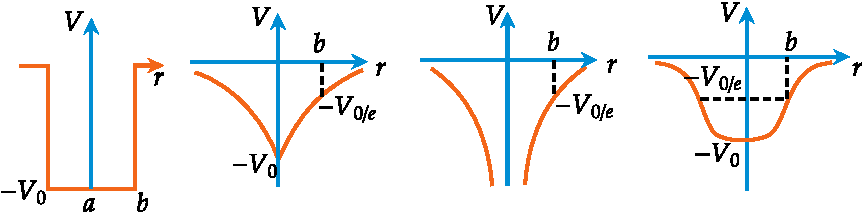
\includegraphics[height=3cm,width=12cm]{diagram-20220309(1)-crop}
		\caption{The four forms of nucleons potential:(a)Rectangular potential (b)Exponential potential(c)Yukawa potential (d)Wools-saxon potential well}
		\label{}
	\end{figure}
\end{enumerate}
 \section{The exchange force model}
 \begin{enumerate}
 	\item There are two principal arguments in support of the presence of exchange forces in nuclei. The first comes from the saturation of nuclear forces. The experimental support for saturation comes from the relatively constant nuclear density and binding energy per nucleon as we go to heavier nuclei. A given nucleon seems to attract only a small number of near neighbors, but it also repels at small distances to keep those neighbors from getting too close.
 	\item Another argument in favor of the exchange force model comes from the study of $\mathrm{np}$ scattering at high energies. There is a strong peak in the cross section at forward angles near $\theta^{\circ}$. corresponding to a small momentum transfer between the projectile and the target. 
 	\item In summary, both the saturation of nuclear forces and the strong backward peak in np scattering are explained by exchange forces. In the former case. "something" is exchanged between nucleons to produce a sort of saturated bond. In the second case. "something" is exchanged between nucleons and actually changes their character.
 	\item according to quantum field theory. the first object does not set up a classical field throughout space but instead emits field quanta. The second object can then absorb those field quanta (and reemit them back to the first object). The two objects interact directly with the exchanged field quanta and therefore indirectly with each other.
 	\item In view of the preceding statement, it is natural to associate the "something" that is exchanged in the nucleon-nucleon interaction with quanta of the nuclear field. For a spin- $\frac{1}{2}$ neutron to turn into a spin- $\frac{1}{2}$ proton, it is clear that the exchanged particle must have integral spin $(0$ or 1$)$ and must carry electric charge.
 	\item  Let us assume that a nucleon (which we denote by $N$, to include both neutrons and protons) emits a particle $X$. A second nucleon absorbs the particle $X$ :
 	$$
 	\begin{aligned}
 	\mathrm{N}_{1} & \rightarrow \mathrm{N}_{1}+\mathrm{X} \\
 	\mathrm{X}+\mathrm{N}_{2} & \rightarrow \mathrm{N}_{2}
 	\end{aligned}
 	$$
 	\item How is it possible for a nucleon to emit a particle of mass energy $m_{x} c^{2}$ and still remain a nucleon, without violating conservation of energy? It is not possible, unless the emission and reabsorption take place within a short enough time $\Delta t$ that we are unaware energy conservation has been violated. Since the limits of our ability to measure an energy (and therefore to determine whether energy is conserved) are restricted by the uncertainty principle, if $\Delta t<\hbar /\left(m_{\mathrm{r}} c^{2}\right)$, we will be unaware that energy conservation has been violated by an amount $\Delta E=m_{x} c^{2}$. The maximum range of the force is determined by the maximum distance that the particle $\mathrm{x}$ can travel in the time $\lambda t$. If it moves at speeds of the order of $c$. then the range $R$ can be at most 
 	$$R=c \Delta_{t}=\frac{\hbar c}{m_{x} c^{2}}$$
 	\item Such particles that exist only for fleeting instants and allow us to violate conservation of energy (and momentum-the emitting and absorbing nucleons do not recoil) are known as virtual particles. We can observe the force that results from the exchange of virtual particles. but we cannot observe the particles themselves during the exchange.
 	\item The exchanged particles that carry the nuclear force are called mesons (from the Greek " meso" meaning middle. because the predicted mass was between the masses of the electron and the nucleon). The lightest of the mesons, the $\pi$-meson or simply pion, is responsible for the major portion of the longer range (1.0 to $1.5$ $\mathrm{fm}$ ) part of the nucleon-nucleon potential. To satisfy all the varieties of the exchanges needed in the two-nucleon system. there must be three pions, with electric charges of $+1,0$, and $-1$. The pions have spin 0 and rest energies of $139.6 \mathrm{MeV}$ (for $\pi^{\pm}$) and $135.0 \mathrm{MeV}$ (for $\left.\pi^{0}\right)$. At shorter ranges $(0.5-1.0 \mathrm{fm}$ ),two-pion exchange is probably responsible for the nuclear binding; at much shorter ranges $(0.25 \mathrm{fm})$ the exchange of $\omega$ mesons $\left(m c^{2}=783 \mathrm{MeV}\right)$ may contribute to the repulsive core whereas the exchange of $\rho$ mesons $\left(m c^{2}=769\right.$ $\mathrm{MeV})$ may provide the spin-orbit part of the interaction.
 \end{enumerate}
\newpage
\begin{abox}
	Practice set 1
	\end{abox}
\begin{enumerate}
	\item The range of the nuclear force between two nucleons due to the exchange of pions is $1.40 \mathrm{fm}$. If the mass of pion is $140 \mathrm{MeV} / \mathrm{c}^{2}$ and the mass of the rho-meson is $770 \mathrm{MeV} / \mathrm{c}^{2}$, then the range of the force due to exchange of rho-mesons is
{\exyear{NET JUNE 2017}}
\begin{tasks}(2)
	\task[\textbf{A.}](a) $1.40 \mathrm{fm}$
	\task[\textbf{B.}]$7.70 \mathrm{fm}$
	\task[\textbf{C.}]$0.25 \mathrm{fm}$
	\task[\textbf{D.}]$0.18 \mathrm{fm}$
\end{tasks}
\end{enumerate}
\newpage
\begin{abox}
	Practice set 2
	\end{abox}
\begin{enumerate}
\item The ground state wavefunction of deuteron is in a superposition of $s$ and $d$ states. Which of the following is NOT true as a consequence?
{\exyear{GATE 2010}}
\begin{tasks}(2)
	\task[\textbf{A.}] It has a non-zero quadruple moment 
	\task[\textbf{B.}]The neutron-proton potential is non-central
	\task[\textbf{C.}] The orbital wavefunction is not spherically symmetric
	\task[\textbf{D.}]The Hamiltonian does not conserve the total angular momentum
\end{tasks}
\item Deuteron has only one bound state with spin parity $1^{+}$, isospin 0 and electric quadrupole moment $0.286 \mathrm{efm}^{2}$. These data suggest that the nuclear forces are having
{\exyear{GATE 2012}}
\begin{tasks}(2)
	\task[\textbf{A.}] only spin and isospin dependence
	\task[\textbf{B.}] no spin dependence and no tensor components
	\task[\textbf{C.}]spin dependence but no tensor components
	\task[\textbf{D.}]spin dependence along with tensor components
\end{tasks}
\item Which of the following statements is NOT correct?
{\exyear{GATE 2016}}
\begin{tasks}(2)
	\task[\textbf{A.}] A deuteron can be disintegrated by irradiating it with gamma rays of energy $4 \mathrm{MeV}$.
	\task[\textbf{B.}] A deuteron has no excited states.
	\task[\textbf{C.}] A deuteron has no electric quadrupole moment.
	\task[\textbf{D.}] The ${ }^{1} S_{0}$ state of deuteron cannot be formed.
\end{tasks}	
\end{enumerate}